% python classes clides - containers and files
% (c) 2012 Kostiantyn Danylov aka koder 
% koder.mail@gmail.com
% distributed under CC-BY licence
% http://creativecommons.org/licenses/by/3.0/deed.en

\documentclass{article}
% XeLaTeX
\usepackage{xltxtra}
\usepackage{xunicode}
\usepackage{listings}
\usepackage[landscape]{geometry}

% Fonts
\setmainfont{DejaVu Sans} %{Arial}
\newfontfamily\cyrillicfont{Nimbus Roman No9 L} %{Arial}
\setmonofont{Courier New}
%\setmonofont{Ubuntu Mono}

%\setmonofont{DejaVu Sans Mono}

% Lang
\usepackage{polyglossia}
\setmainlanguage{russian}
\setotherlanguage{english}
\usepackage[dvipsnames,table]{xcolor}


\ifx\pdfoutput\undefined
\usepackage{graphicx}
\else
\usepackage[pdftex]{graphicx}
\fi

\lstset{
	language=python,
	keywordstyle=\color{Emerald},%\texttt, 
	commentstyle=\color{OliveGreen},%\texttt,
	stringstyle=\color{Bittersweet},%\texttt,
	tabsize=4,
	numbers=left,
	xleftmargin=10pt,
	morekeywords={with,as},	
	numberstyle=\large,
	%identifierstyle=\texttt,
	%basicstyle=\texttt,
}

\usepackage{hyperref}

\hypersetup{
	colorlinks=true,
	urlcolor=blue
}

\usepackage{float}
%\floatstyle{boxed} 
%\restylefloat{figure}
\usepackage[normalem]{ulem}

\input{files/python_cmds}
\begin{document}
\LARGE

%-------------------------------------------------------------------------------
\begin{center} Контейнеры \end{center}
\begin{itemize}
	\item Массив(список) list
	\item Константный массив(кортеж) tuple
	\item Словарь dict
	\item Множество set
	\item frozenset, buffer, ....
\end{itemize}
\begin{lstlisting}
	[1, 2, 3]
	(1, 2, 3)
	{1:"1", 2:"2", 3:"3"}
	{1, 2, 3}
\end{lstlisting}
\newpage

%-------------------------------------------------------------------------------
\begin{center} list – Список (Массив) \end{center}
\begin{itemize}
	\item Упорядоченное множество элементов, доступ по номеру
	\item \lstinline!var = [1, 2, 3]!
	\item Индексация \lstinline!arr[x]!
	\item Срезы 
			\lstinline!arr[frm:to:step]! \\
			\lstinline![arr[frm], arr[frm + step], ....., ]!
	\item Отрицательный индекс - отсчет от конца к началу. x[-1]
	\item Отсутвие индекса - frm $\rightarrow$ 0, to $\rightarrow$ \lstinline!len(x)!, 
	        step $\rightarrow$ 1
\end{itemize}
\newpage

%-------------------------------------------------------------------------------
\begin{center} list – Список (Массив) \end{center}
{
\Huge
$x = [0_{-6}^{0}, 1_{-5}^{1}, 2_{-4}^{2}, 3_{-3}^{3}, 4_{-2}^{4}, 5_{-1}^{5}]$ \\
\vspace{1cm}
\begin{tabular}{ l l l }
x[2] & == 2 & \hspace{2cm}[\textcolor{red}{0, 1,} 2, \textcolor{red}{3, 4, 5}] \\
x[-2] & == 4 & \hspace{2cm}[\textcolor{red}{0, 1, 2, 3,} 4, \textcolor{red}{5}] \\
x[2:] & == [2, 3, 4, 5] & \hspace{2cm}[\textcolor{red}{0, 1, }2, 3, 4, 5] \\
x[-2:] & == [4, 5] & \hspace{2cm}[\textcolor{red}{0, 1, 2, 3,} 4, 5] \\
x[1:-1] & == [1, 2, 3, 4] & \hspace{2cm}[\textcolor{red}{0,} 1, 2, 3, 4, \textcolor{red}{5}] \\
x[1:-1:2] & == [1, 3] & \hspace{2cm}[\textcolor{red}{0,} 1, \textcolor{orange}{2,} 3, \textcolor{orange}{4,} \textcolor{red}{5}] \\
x[1:-1:-2] & == [4, 2] & \hspace{2cm}[\textcolor{red}{0,} \textcolor{orange}{1}, 2, \textcolor{orange}{3}, 4, \textcolor{red}{5}] \\
x[::-1] & == [5, 4, 3, 2, 1, 0] & \\
\end{tabular}
}
\newpage

%-------------------------------------------------------------------------------
\begin{center} list – Операции нам элементам и срезам \end{center}
\vspace{15pt}
\begin{lstlisting}
	x = [3, 4, 5, 6]
	range(x) == [0, ..., x – 1]
	range(x, y, z) ~= range(INF)[x:y:z]

	x[::2] = [2, 2]  
	x == [2, 4, 2, 6]
	x[::2] = 2 # TypeError
	x[:2] = [7] # x == [7, 2, 6]
	
	del x[1] # x == [7, 6]
	
	x = [1, None, True, ["123", 2.4]]
	[1, 2, 3] + ["a", "b"] # [1, 2, 3, "a", "b"]
\end{lstlisting}
\newpage

%-------------------------------------------------------------------------------
\begin{center} Методы списка \end{center}
\begin{Large}
\vspace{15pt}
\begin{lstlisting}
	# arr.append(val)
	[1, 2].append(3) => [1, 2, 3]

	# arr.extend(arr2)
	[1, 2].extend([2, 3]) => [1, 2, 2, 3]

	# arr.pop()
	x = [1, 2]
	x.pop() == 2
	x == [1]

	# arr.insert(pos, val)
	[1, 2].insert(0, "abc") => ["abc", 1, 2]

	[1, 2].index(2) => 1
	[1, 2].reverse() => [2, 1]
	[1, 2, 4, 1, 2, 4, 1, 1].count(1) == 4
	x = [1, 3, 2]
	x.remove(1) # x == [3, 2]
	x.sort() # x == [2, 3]
\end{lstlisting}
\end{Large}
\newpage

%-------------------------------------------------------------------------------
\begin{center} Изменяемые типы (ссылочные) \end{center}
\vspace{15pt}
\begin{lstlisting}
	x = [1, 2, 3]
	y = x
	y.append(1)
	print x => [1, 2, 3, 1]
\end{lstlisting}
\newpage

%-------------------------------------------------------------------------------
\begin{center} Изменяемые типы (ссылочные) \end{center}
\begin{lstlisting}
	x = [["1"], "2"]
	y = x
\end{lstlisting}
\includegraphics[scale=0.8]{images/refs1.eps}

\begin{lstlisting}
	x = [["1"], "2"]
	y = x[:]
\end{lstlisting}
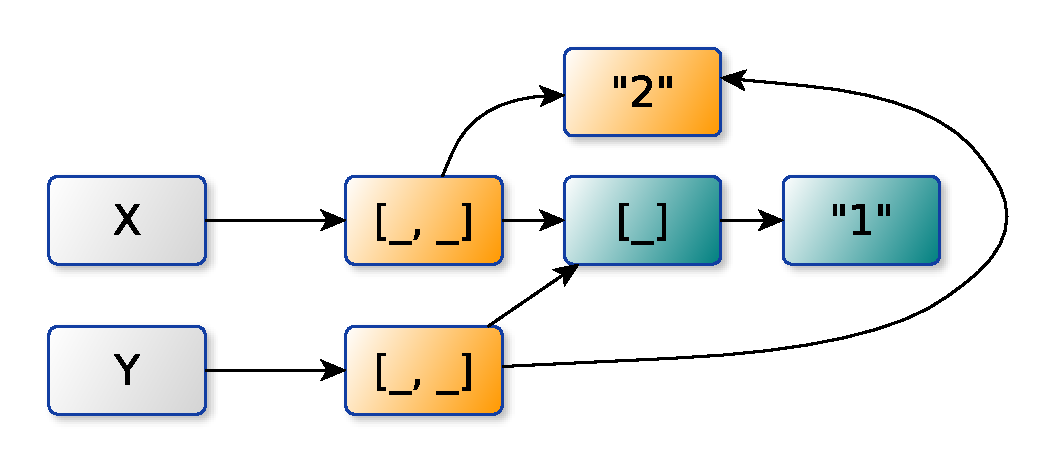
\includegraphics[scale=0.8]{images/refs2.eps}
\newpage

\begin{lstlisting}
	import copy
	x = [["1"], "2"]
	y = copy.deepcopy(x)
\end{lstlisting}
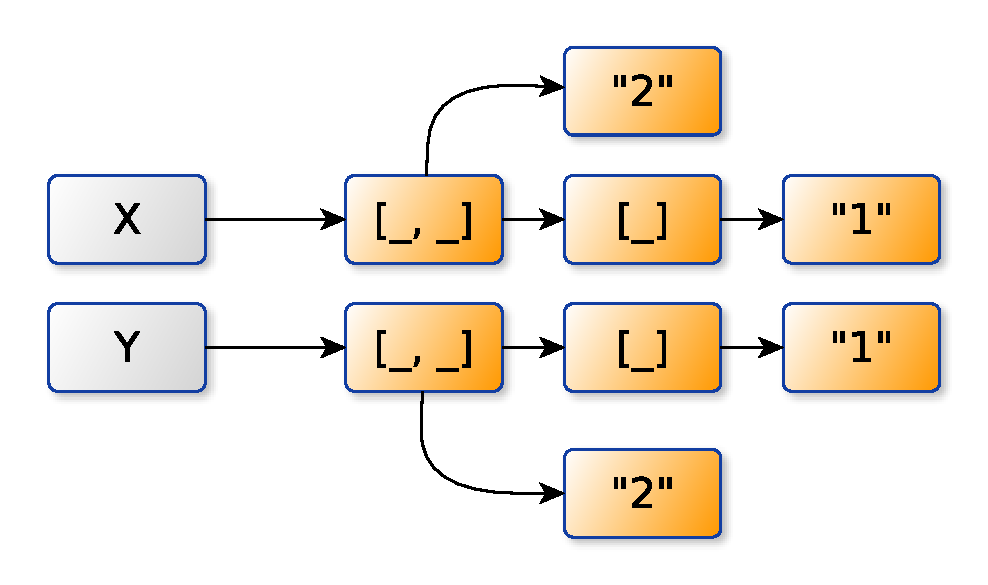
\includegraphics[scale=0.8]{images/refs3.eps}

\newpage

%-------------------------------------------------------------------------------
\begin{center} Сортировка \end{center}
\begin{itemize}
	\item sort() сортировка на месте, sorted - возвращает копию
	\item Не надо сортировать неоднородные контейнеры типы - результат не определен
		По больше части - получится что-то, но иногда -
		\lstinline!['x', '\xf0', u'x'].sort()! - UnicodeDecodeError
\end{itemize}
\begin{lstlisting}
	x = [2, 3, 4, 1 , 6, -2]
	sorted(x) == [-2, 1, 2, 3, 4, 6]
	x == [2, 3, 4, 1 , 6, -2]
	x.sort()
	x == [-2, 1, 2, 3, 4, 6]
\end{lstlisting}
\newpage

%-------------------------------------------------------------------------------
\begin{center} tuple – кортеж \end{center}
\begin{itemize}
	\item Константный список (но можно изменять элементы, если они не константные)
	\item Предназначается для небольших коллекций разнородных элементов
\end{itemize}
\vspace{15pt}
\begin{lstlisting}
	tpl = (1, 2)
	tpl = 1, 2
	tpl[1] = 3 # TypeError
	tpl = (1, [2, 3, 4])
	tpl[1].append(1) => (1, [2, 3, 4, 1])
	x, y, z  = (1, 2, 3)

	(1) == 1
	(1,) == (1,)
\end{lstlisting}
\newpage

%-------------------------------------------------------------------------------
\begin{center} dict - словарь \end{center}
\begin{itemize}
	\item Набор пар (ключ, значение), с быстрым поиском по ключу
	\item Только константные ключи (tuple - ok)
	\item Элементы неупорядоченны
	\item Нет срезов
\end{itemize}
\vspace{15pt}
\begin{lstlisting}
    x = {1:2, "3":4}
	x[1] == 2
	x[2] # KeyError
	1 in x == True
	x[17] = True
	x == {1:2, "3":4, 17:True}
\end{lstlisting}
\newpage

%-------------------------------------------------------------------------------
\begin{center} dict – Словарь \end{center}
\vspace{15pt}
\begin{lstlisting}
	x = {1:2, "3":"4"}
	dict(a=1, b=2) == {"a":1, "b":2}
	x.items() == [(1, 2), ("3", "4")]
	x.values() == [2, "4"]
	x.keys() == [1, "3"]
	x.copy() == {1:2, "3":"4"}
	x.setdefault(key, val) == val
	x.get(5) == None
	x.get(5, 12) == 12
	x.clear() # {}
	x.update(y)
	dict.fromkeys(keys, val) 
	# {key[0]:val, key[1]:val, ..} default val is None
\end{lstlisting}
\newpage

%-------------------------------------------------------------------------------
\begin{center} set - множество \end{center}
\begin{itemize}
	\item Множество элементов с быстрым поиском и операциями
\end{itemize}
\vspace{15pt}
\begin{lstlisting}
	x = {1, 2} 
	y = set([2, "a"]) # y == {2, "a"}
	x & y == x.intersection(y) == {2}
	x – y == x.difference(y) == {1}
	x | y == x.union(y) == {1, 2, "a"}
	x.issubset(y) # ....

	set(1, 2, 3) # error
	set("abcd") == set(["a", "b", "c", "d"])
\end{lstlisting}
\newpage

%-------------------------------------------------------------------------------
%level=3
\begin{center} Особенности поведения set \& dict \end{center}
\begin{itemize}
	\item Ключи сравниваются с помощью hash, затем ==
	\item \lstinline!hash(2.0) == 2, hash(2) == 2, 2.0 == 2!
	\item Для пользовательских объектов hash \& == можно перегрузить
\end{itemize}
\begin{lstlisting}
	{2.0: "ccc", 2: "dd"} == {2.0: "ccc"}
	set([2]) | set([2.0]) == set([2])
	set([2.0]) | set([2]) == set([2.0])
	set([2]) == set([2.0])
\end{lstlisting}
\newpage

%-------------------------------------------------------------------------------
\begin{center} Общие операции над контейнерами \end{center}
\begin{itemize}
	\item Пребразование к list, tuple, set
	\item len - количество элементнов
	\item str.join \lstinline!", ".join(["1", "2", "3"]) == "1, 2, 3"! 
	\item in проверка включения элемента
	\item Проеобразование контейнера пар к словарю 
\end{itemize}
\begin{lstlisting}
    y = [1, 2, 3]
    set(y) == {1, 2, 3}
    tuple(y) == (1, 2, 3)
    set(1, 2, 3) # TypeError
	x = [(1, "1"), (2, "2")]
	dict(x) == {1:"1", 2:"2"}
\end{lstlisting}
\newpage

%-------------------------------------------------------------------------------
\begin{center} heapq \end{center}
Массив, где $x_n >= x_{2n}, x_n >= x_{2n + 1}$
\begin{lstlisting}
    x = [2, 4, 5, 3, 8, 1, 7, 9, 0, 6]
    heapq.heapify(x)
    x == [0, 2, 1, 3, 6, 5, 7, 9, 4, 8]
    tuple(y) == (1, 2, 3)
    set(1, 2, 3) # TypeError
	x = [(1, "1"), (2, "2")]
	dict(x) == {1:"1", 2:"2"}
\end{lstlisting}
\newpage

%-------------------------------------------------------------------------------
\begin{center} Ассимптотика контейнеров \end{center}
\begin{center}
\begin{tabular}{ | l | l | l | l | l | }
	\hline
       & \cellcolor[gray]{0.8} list/tuple & \cellcolor[gray]{0.8} dict/set &  \cellcolor[gray]{0.8} sorted list & \cellcolor[gray]{0.8} heap \\
  	\hline
  insert/remove begin     & \cellcolor{pink} $O(n)$ & \cellcolor{green} $O(1)^*$ & \cellcolor{pink} $O(n)$ & \cellcolor{Aquamarine} $O(log(n))$ \\
  	\hline
  insert/remove end       & \cellcolor{green} $O(1)$ & \cellcolor{green} $O(1)^*$ & \cellcolor{green} $O(1)$ & ---  \\
  	\hline
  find by key      &  --- & \cellcolor{green} $O(1)^*$ & --- & --- \\
  	\hline
  find by value     &  \cellcolor{pink} $O(n)$ & \cellcolor{pink} $O(n)$ & \cellcolor{Aquamarine} $O(log(n))$ & \cellcolor{pink} $O(n)$ \\
  	\hline
  find min/max     &  \cellcolor{pink} $O(n)$ & \cellcolor{pink} $O(n)$ & \cellcolor{green} $O(1)$ & \cellcolor{green} $O(1)$/\cellcolor{pink} $O(n)$ \\
  	\hline

\end{tabular}
\end{center}
\newpage

%-------------------------------------------------------------------------------
\begin{center} Сборка мусора \end{center}
\begin{itemize}
	\item С каждым объектом связан счетчик ссылок
	\item Счетчик инкрементируется при появлении каждой новой ссылки на объект:
	       переменной, помещения в контейнер, etc
	\item И декрементируется при каждом исчезновении ссылки
	\item Как только счетчик оказывается равен нулю - объект удаляется
\end{itemize}
\newpage

%-------------------------------------------------------------------------------
\begin{center} Сборка мусора \end{center}
\begin{center} 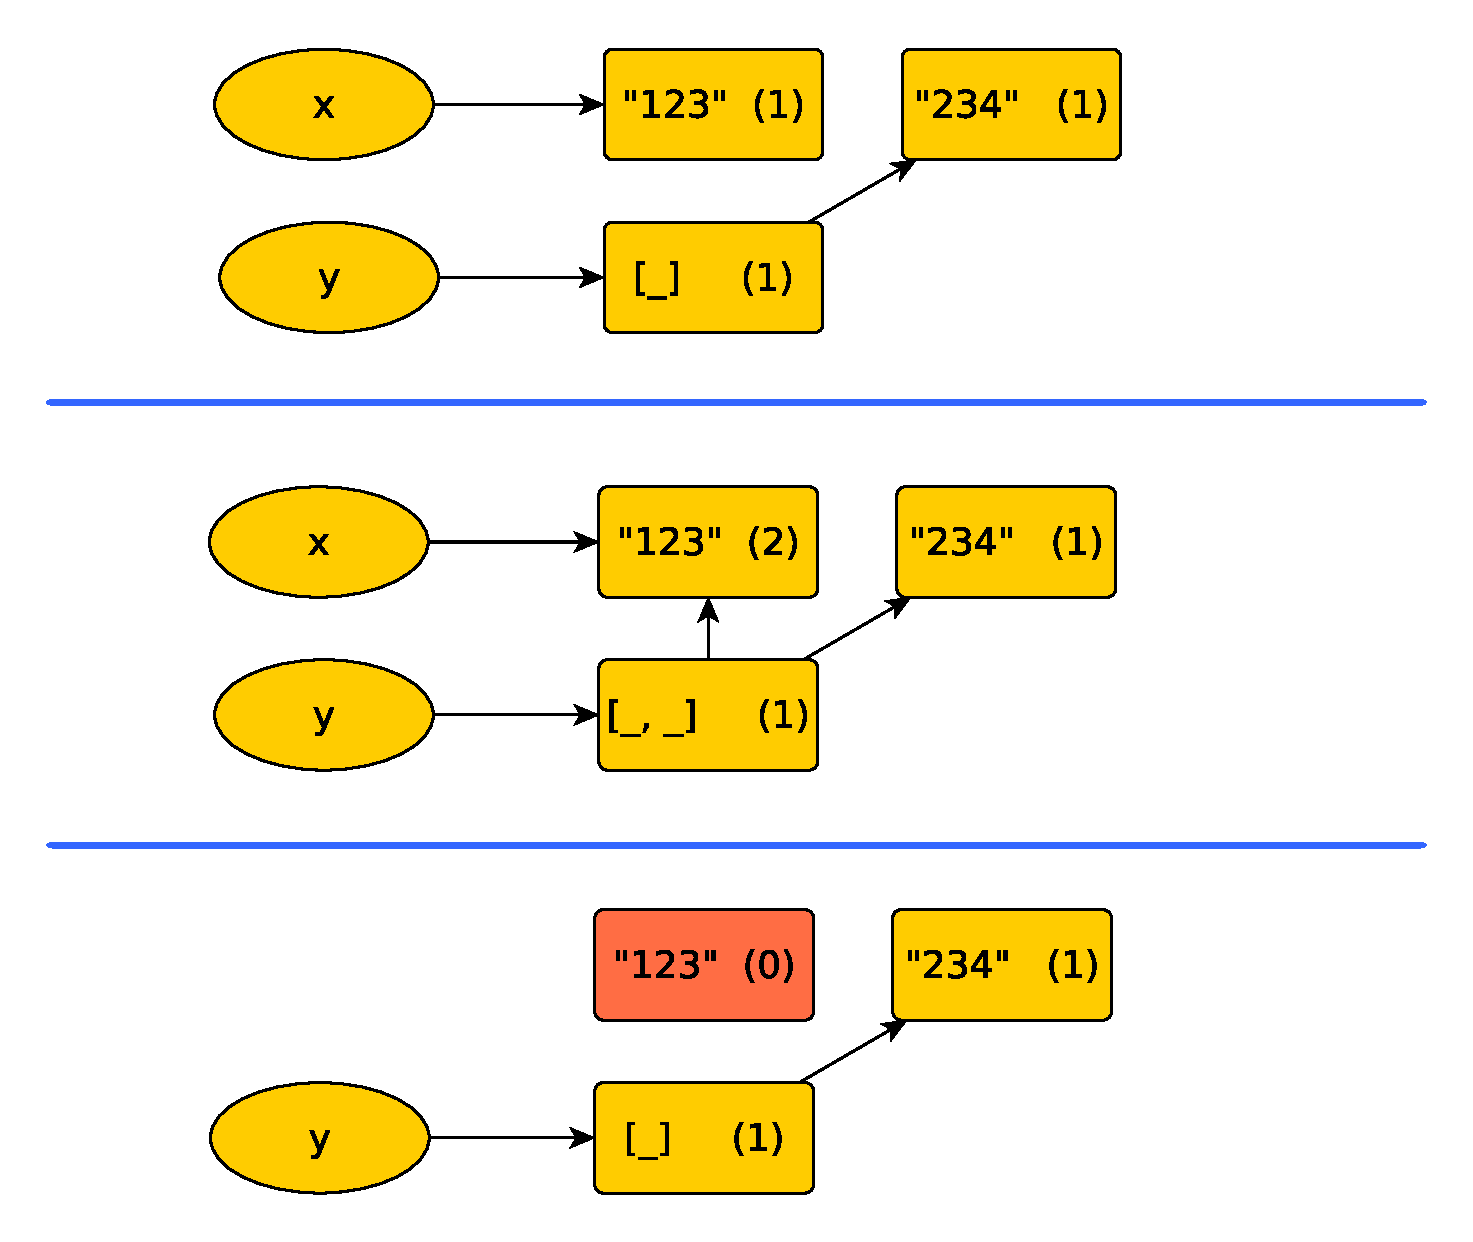
\includegraphics[scale=0.6]{images/ref_counter.eps}\end{center}
\newpage

%-------------------------------------------------------------------------------
\vspace{15pt}
Циклические ссылки не удаляются автоматически. Такие объекты остаются в памяти до
запуска сборщика мусора.
\begin{lstlisting}
	a = []
	a.append(a)

	a = []
	b = []
	a.append(b)
	b.append(a)
\end{lstlisting}
\begin{center} 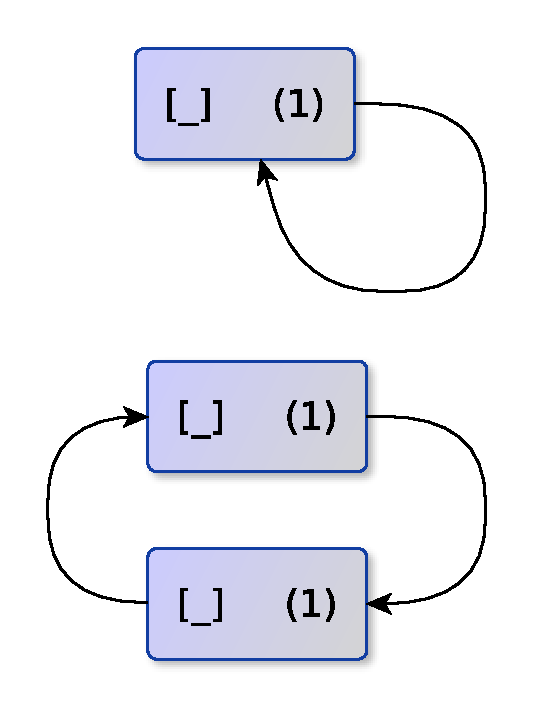
\includegraphics[scale=0.6]{images/cycle_ref.eps}\end{center}
\newpage

%-------------------------------------------------------------------------------
\begin{center} Файлы \end{center}
\begin{itemize}
	\item Абстракция для источников или приемников данных
	\item Тестовые и бинарные
	\item Поддерживается запись/чтение/позиционирование/os.ioctl
	\item open(name, mode) - открывает файл
	\item read([len]) - читает данные. При окончании данных возвращает ""
	\item write(string) - пишет данные
	\item seek, tell, readline, readlines
\end{itemize}
\newpage

%-------------------------------------------------------------------------------
\begin{center} Файлы \end{center}

\begin{lstlisting}
	import os

    fd = open(path, mode)
    mode in {"r", "w", "r+", "a", 
             "rb", "wb", "rb+", "ab"}
	fd.read(size) # data str
	fd.write("data")
	fd.seek(pos, frm)
	
	# frm in {os.SEEK_SET, os.SEEK_CUR, os.SEEK_END}
	
	fd.read() # till the end
	fd.readline() # untill "\n"
\end{lstlisting}
\newpage

%-------------------------------------------------------------------------------
\begin{center} Файлы \end{center}
Можно итерировать по строкам:
\begin{lstlisting}
	import os

    fd = open(path)
    for line in fd:
        	# do something with line
\end{lstlisting}
\newpage

%-------------------------------------------------------------------------------
\begin{center} Файлы 3.X \end{center}
\begin{lstlisting}
    fd = open(path, "r", encoding='utf-8')
	fd.read(size) # unicode str

    fd = open(path, "rb")
	fd.read(size) # bytes
\end{lstlisting}
Модуль io содержит дополнительные классы для работы с воодом-выводом
\newpage

%-------------------------------------------------------------------------------
\end{document}
